\chapter{Practical Implementation}

\section{Dataset selection}

\section{Data preparation}

	\subsection{Data processing and data wrangling}
	\lstinputlisting[
	label=code:WhileLoop,    % Label; genutzt für Referenzen auf dieses Code-Beispiel
	caption=Algorithmus zum Schätzen einer Zahl in Python,
	captionpos=b,               % Position, an der die Caption angezeigt wird t(op) oder b(ottom)
	style=EigenerPythonStyle,   % Eigener Style der vor dem Dokument festgelegt wurde
	firstline=0,                % Zeilennummer im Dokument welche als erste angezeigt wird
	lastline=23                 % Letzte Zeile welche ins LaTeX Dokument übernommen wird
	]{Quellcode/json-schema.json}
	
	\subsection{Data cleaning}
	
	\subsection{Considerations of Space and Time Complexity}
	The dataset consists of over 150.000 invoices, and in those invoices, over 350.000 items are listed. 
	With hardware-limitation in place, an optimized approach for storing and processing the data is required. 
	Several considerations for speeding up processing time and reducing storage space can be made. 
	In the following, the observations are explained and approaches for improvement are given.

		\subsubsection{Duplicates and space complexity}
		Investigation shows, there are only 79.741 unique descriptions for the listed items. By saving only the unique values, the required space is reduced to less than one fourth compared to before. Additionally, this step is required by most machine learning models, as duplicate input values can skew the outcome. The model is chosen later, so this processing step leaves the model selection more open to different kinds of learning algorithms.
		
		\subsubsection{Reconstructing Relationships and time complexity of searching}
		After the deletion of duplicate descriptions (documents in the corpus), the 
		
		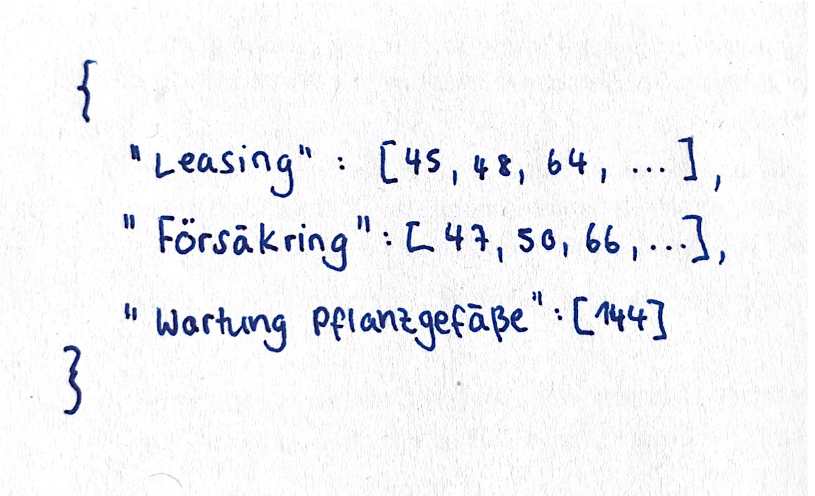
\includegraphics[height=8cm]{Bilder/description_map.png}

	\subsection{Feature Extraction and Feature Engineering}

\section{Modelling}
\section{Evaluation}
	\subsection{Visualization}
\section{Deployment}